\chapter{Real-time processing in the Big Data context [VI]}
\label{chap:real_time_processing}

Many information systems today require fast or even instant response to a coming data.
When new peace of data arrives into the system from a user, outer sensor, or any other source, system must reflect change of its state quickly. 
The batch processing, that we describe in the Chapter~\ref{chap:google_architecture}, can not fulfil this requirement, because it takes usually long time to execute.
The real-time processing allows to do that.

Necessity of response to a coming data fast is especially applicable to the Web world.
Companies like Google, Twitter, LinkedIn, Facebook, etc. process not just much of data, but also often need to do it quickly.
This, in fact, brings to a simultaneous use of both types of processing in one system.

We already described the batch processing and the MapReduce paradigm as its application.
It has two considerable advantages.
First of all, it is very efficient.
It fetches batches of data, and processs them at once, what is always faster, than taking records arbitrarily one by one.
Another advantage is that it allows to execute on data any function we have in mind, as long as all data is at the disposal.
When we have data coming from the stream record by record, this is not possible.
In that case we have to create alternative methods to apply the same algorithms.
Usually they become approximated, and accuracy is a matter of tradeoff.

To define the real-time processing, we need first to explain what is the real time.
There is no such thing in physics as real time, because any event takes time to happen.
But human understands, and even feels, that one event takes long time, but another is happening ``instanlty''.
This is of course only a matter of our perception.
We are not able to differentiate intervals smaller than parts of a second.
As a result, we define real time as an interval of time that short enough in the current context.
In some cases it is seconds or minutes, but sometimes even milliseconds, and then things become really interesting.

The real-time processing is then processing of the data, that takes time, short enough in the current context.
Let us consider two examples.
The first is a page visits counter.
It does not require any super fast reflection of how many people visited the page, and as a result, system can update it once in a minute, aggregating all visit events during this time.
Real time is a minute in this case.
Another example is an alarm system at the nuclear powerplant.
It must monitor the state of the whole plant, and process all data, coming from many temperature sensors, to report about danger case and to switsch defence mechanisms as fast as possible.
Here real time is milliseconds.

Execution of the real-time processing using standard methods and algorithms is not possible.
We do not have all data at the disposal, what is always much simpler, than to process data in pieces.
There are many specific algorithms for the real-time data processing.
They usually differ quite much from batch algorithms, because of the nature of input they consider.
They divide to different categories depending on what type of query do they answer.
A few query types are: ``has an item already been observed in the stream?'', ``how many times has an item been observed in the stream?'', ``what is the number of unique items among observed in the stream?'', etc.
We discuss the real-time processing algorithms further in this chapter in more technical details.

\section{Examples from real life}

Describe several examples how well-known companies apply real-time processing to the real data.
What algorithms do they maybe use, what topology or schema of computations in general.

The real
Many companies as well as 

Twitter uses real time processing immensely \cite{Toshniwal2014} \cite{Boykin2013}.


\section{Sketch Algorithms for Estimation of Stream Parameters [VI]}

To create aggregations, indexes and views of data, coming from the stream, we have often to answer different mathematical questions.
For example: ``has a particular item already been observed in the stream?'', ``how many times specific item has already arrived from the stream?'', ``what is the cardinality of the set of items so far observed in the stream?'', etc.
We can represent all these questions in a mathematical way, in the form of sets, values and functions.

To answer such questions stream processing algorithms, or \textit{sketch algorithms}\mnote{sketch algorithm}, exist.
They consider data coming from the stream as a mathematical space of values of a particular type, and compute functions on that space.
The result of those functions is a set of values that gives an opportunity to answer particular query.

Sketch algorithm receives data from the stream and continuously builds the \textit{sketch}\mnote{sketch}.
Sketch is a data structure that persists only the part of information that stream produces.
It is always compact and stores not original values from the stream, but specific type of aggregation.

In comparison with the amount of original data, sketch algorithm uses small amount of memory to maintain sketch.
Sketch is usually a variation of hash-table or combination of several hash-tables.
It allows answering particular query fast, mostly in a constant time, that does not depend on the size of the sketch.

Sketch algorithm produces usually only approximated result.
This is logical, because it condenses data set coming from the stream.
Technically speaking, it answers query with error that is the function of algorithm's parameters.
For example, if the answer to the query is a Boolean answer (yes or no), wrong answer can occur with some probability.
If the answer is a number, deviation from exact right value is possible.

\subsection{Bloom Filter}

The Bloom filter answers query ``has a particular item been observed in the stream?'' \cite{Cormode}.
It works in a constant time and requires small amount of memory to hold.
It has several parameters that affect its size, time of request and rate of error.

The Bloom filter is essentially a hash-table, but it does not store elements themselves.
Instead, it is internally a bitset.
It uses several hash-functions, so that when we put new element into the Bloom filter, it computes hash-values using each hash-function, interpret them as indices, and put 1 by each of them.
To query an element, it does the same thing; it computes all hash-functions, and checks, whether all positions are equal to 1.
If so, the Bloom filter answers ``yes'', and it can be false positive, because hash-functions produce collisions.
We can adjust rate of false positives, changing parameters of the Bloom filter.
If answers is ``no'', it is always true by definition of the filter.
Figure~\ref{fig:bloom_filter} depicts the inner state and the way of requests to the Bloom filter.

\begin{figure}[h]
  \centering
  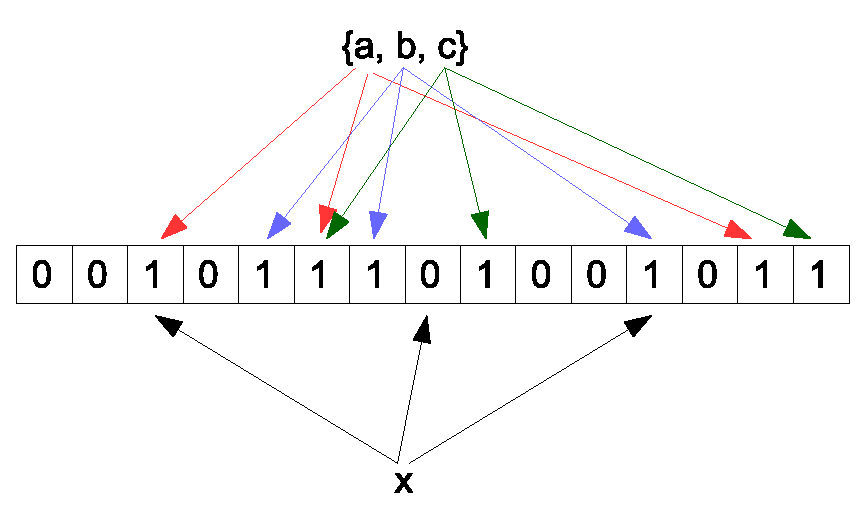
\includegraphics [width=0.6\textwidth]{images/BloomFilter}
  \caption{The inner state and requests to the Bloom filter.}
  \label{fig:bloom_filter}
\end{figure}

The Bloom filter has three parameters that affect its properties.
$m$ - the size of the filter, i.e. the number of bits in the bitset.
Its variation defines not only memory usage, but also the rate of false positives, because the more bits are in use, the less probability of collisions.
$k$ - the number of hash-functions.
This parameter influences again the rate of error.
If there are too less hash-functions, probability to encounter bits, set to 1 by other value, gets more.
At the same time, if there too many hash-functions, filter gets full faster, and again, probability to meet all 1 grows.
Also this parameter affects speed of request to the filter, because every additional hash-function requires time to compute.
$n$ - the number of values, already inserted into the filter.
This parameter is not inherent for the filter, but has a dynamic nature, because it depends on the statistical properties of the stream.
Nevertheless, it affects filter's behavior and is to consider.

Next expression describes the rate of false positives as a function of all three parameters discussed

$$
FP\_rate = \Bigg(1 - \Bigg[1 - \frac{1}{m}\Bigg]^{kn}\Bigg)^k \approx \Big(1 - e^{-kn/m}\Big)^k
$$

Having set parameters $m$ and $n$ we can infer the optimal number of hash-functions, that minimizes error rate

$$
k = \frac{m}{n}ln2
$$

Bloom filter is a great algorithm that finds many examples of use.
Early UNIX spell-checkers used the Bloom filter to check spelling fast, prestoring the whole dictionary in the filter \cite{BroderMitzenmacher2005}.
The Bloom filter allows to store all unsuitable passwords, that users are not permitted to choose \cite{BroderMitzenmacher2005}.
Bitcoin uses the Bloom filter to speed up wallet synchronization \cite{BitcoinFoundation2012}.
Google BigTable and Cassandra systems use the Bloom filter to reduce the number of hard disk lookups \cite{Bigtable/Chang_Dean_Ghemawat}.

\subsection{Count-Min Sketch}

The Count-min sketch answers the query ``how many times has an item been observed in the stream?'' \cite{Cormode}.
It gives always estimated value of the number of occurrences of a particular item.
The rate of error is again a matter of adjusting parameters.
The Count-min sketch can only overestimate the result, meaning give a value equal or greater than true frequency.

The Count-min sketch consists of several arrays of counters.
We denote the matrix, that represents it, as $C$.
Matrix $C$ has $d$ rows and $w$ columns.
The number of rows $d$ is at the same time the number of used hash-functions, so that one function corresponds to one row.
The number of columns $w$ is simply a length of the sketch, and it influences accuracy of the algorithm.

The Count-min sketch works in the following way.
When new item $i$ arrives from the stream, sketch computes each hash-function $h_j(i)$.
For $j$-th hash-function it increments the counter (with index equal to $h_j(i)$) in the $j$-th row of the matrix $C$.
So for each item $i$ sketch increments exactly $d$ counters.
Finally, entry of the matrix $C$ has the next form

$$
C[j, k] = \sum_{h_j(i)=k}f(i)
$$

where $f(i)$ is a frequency of an item $i$.
You can see the view of the Count-min sketch on the Figure ~\ref{fig:count_min_sketch}

\begin{figure}[h]
  \centering
  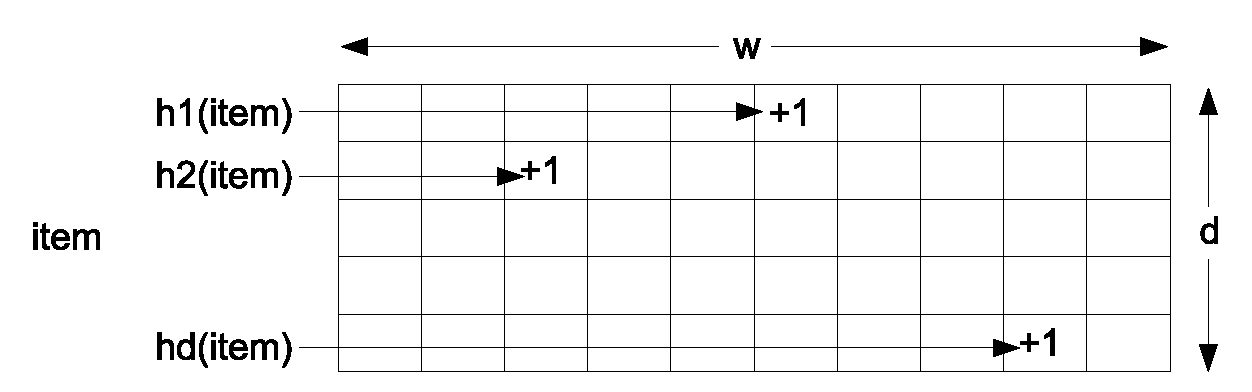
\includegraphics [width=0.6\textwidth]{images/CountMinSketch}
  \caption{The view of the Count-min sketch.}
  \label{fig:count_min_sketch}
\end{figure}

To execute a query, sketch computes again all hash-functions of interesting item $i$, finds all counters, and takes the minimum among them.
As long as collisions can occur, sometimes different items from the stream lead to grow of the same counter in the same row of the matrix.
This can consequently give an overestimation of frequency.
We can reduce the probability of overestimation and its value increasing parameters $d$ and $w$.
The next expression shows frequency estimation for an item

$$
\hat{f}(i) = min_{1 \leq j \leq d}C[j,h_j(i)]
$$

%\subsection{HyperLogLog algorithm}

%The HyperLogLog algorithm answers the query ``how many distinct items have been observed in the stream?''.
%\cite{Heule2013, Flajolet2007}



%\section{Application in the speed layer}

Descirbe how stream processing algorithms can be applied in the speed layer.
How can we build topology to solve some particular task, to creat some aggreagation for example.
How all this works technically, data pipelines, usage of different algorithms.
%anomaly detection